

\subsection{Program Structure}
\label{sec:ProgramStructure}

Now when the operating system is defined, the next stage will be to define the actual application that needs to be implemented. Given the block diagram of figure \ref{fig:TheSystemBlockDiagram}, the blocks that make up the system is already defined.

\subsubsection{Defining tasks}
\label{sec:DefiningTasks}
First step is to identify the tasks that make up the system. A good rule of thumb is to make a driver task for every peace of hardware that the system is to interact with. This idea is based on the Parallel criteria which implies that things can be separated in to different tasks if the functionality runs independent and simultaneously, which indeed will be the case for a hardware driver.
However the UART0 driver that supports connection between the PC and micro controller, can send and receive data independently. Therefore this task is split up in to two tasks. A receive task, and a transmit task.
Doing so also have the advantage of reusability, for other applications requiring the same hardware. 

Now when all the hardware is taken care of, the only thing remaining is the application it self. The application should be able to handle commands given by the user. Commands could be "set coordinate pan, tilt", "run light-show \#2" an "set minimum velocity tilt". Since the entire application will consist of function calls, the main body of the application will take the shape of a kernel task that execytes the functions defined in the function list shown in appendix 
\ref{sec:KernelInstructionList}. However by executing the command "run light show" it require of the application to feed the P\&T driver with new target points once the previus target point has been reached. considering that one still would like to send commands while running a light-show this will make two tasks based on the parallel criteria. The kernel Task and the light-show task.

Last but not least the application operate on the current position in order to handle a light-show. But gaining the current position requires pulling from the application. This task therefore makes the final task in the system based on the Periodical Criteria. 

The application must therefore consist of the following tasks:

Driver tasks:
\begin{itemize}[noitemsep]
	\item UART0\_rx\_task
	\item UART0\_tx\_task
	\item Joystick\_task
	\item SPI\_Master\_task
\end{itemize}

Application tasks:
\begin{itemize}[noitemsep]
	\item app\_kernel\_task
	\item app\_lightshow\_task
	\item app\_update\_current\_task
\end{itemize}	
	
\subsubsection{Connecting the tasks}
Now the tasks are to be linked together. This will happen in a structure so that every task that requires input from other tasks has one and only one queue to pull from. This is decried since the OS can pause the task while waiting for one queue. The UART tasks and the joystick tasks will both send commands to kernel via the application queue, an shared state memory. The same goes for the connection between the kernel task and the light-show task. 

Each queue needs to be semaphore protected in order to prevent a race condition when reading an writing to the queue, but since freeRTOS handles who gets to use the queues, it must be safe to amuse that such conditions is taken care of in the OS. 

The shared state memory (SSM), needs semaphore protection as well. Since the number of memory locations is relatively small (less then 64), combined with the fact that the critical section only consists of one read ore write. the entire SSM will be handled by the same semaphore for simplicity. 



Now when the task diagram has been made, it is time to considerer possible structural weakness such as deadlocks and handling og queues. 

% full dreasd task diagram
\begin{figure}
	\centering
	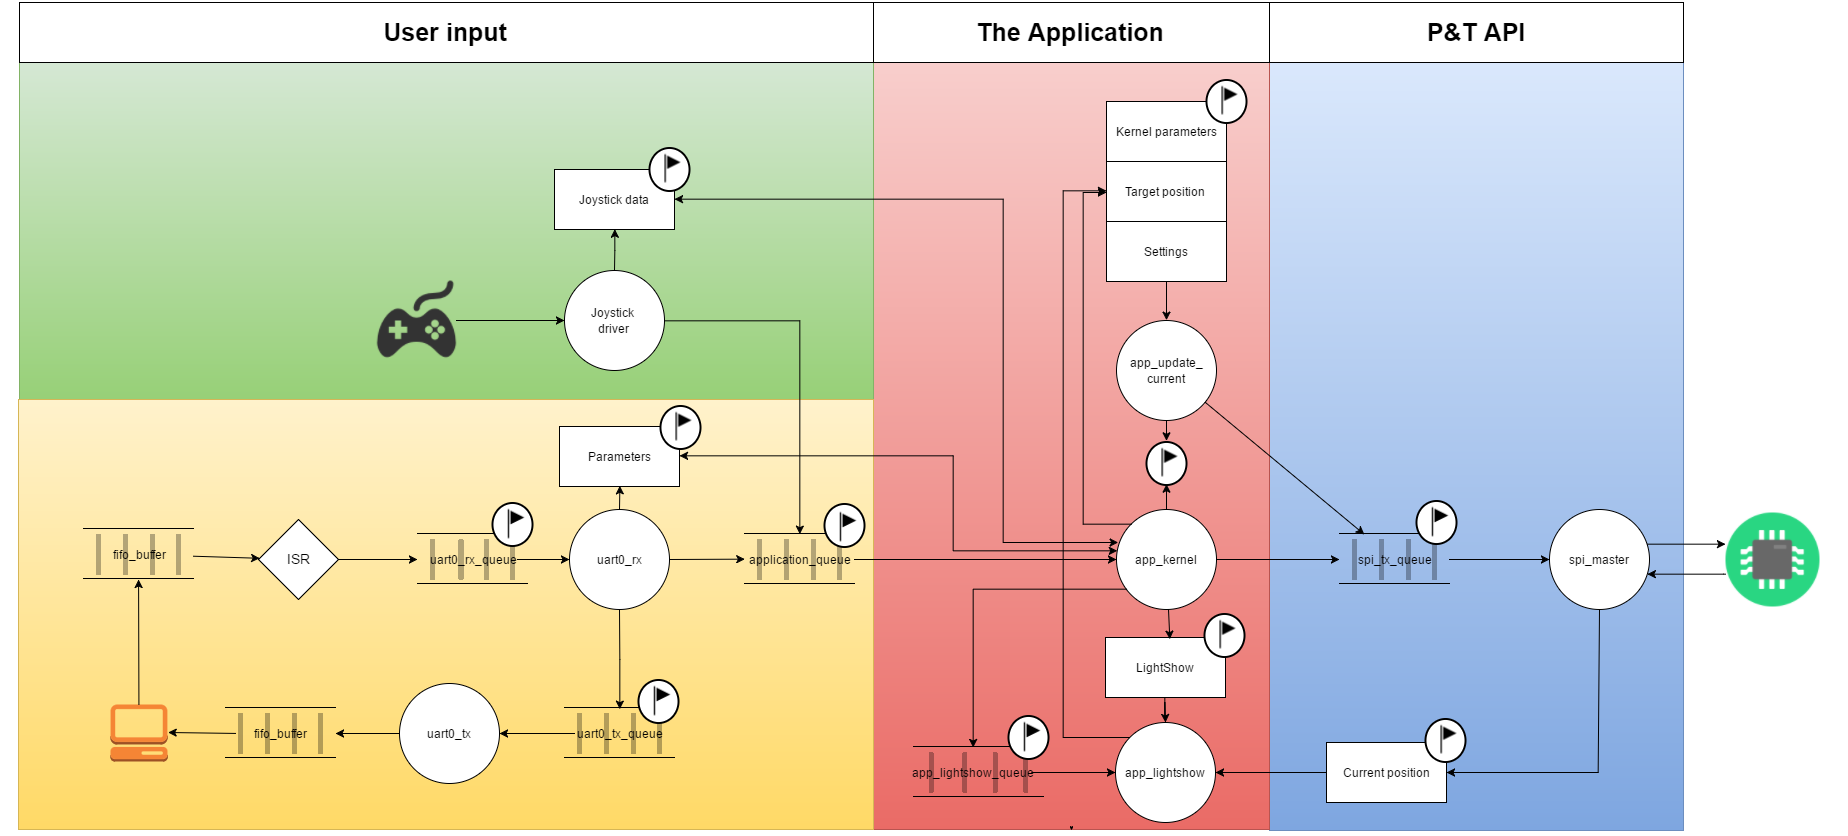
\includegraphics[scale= 0.4, angle = 90] {Billeder/microcontroller-Task-Diagram}
	\caption{The application task diagram}
	\label{fig:applicaiton_task_diagram}
\end{figure}




